\begin{XeClass}{PermissionStatus}
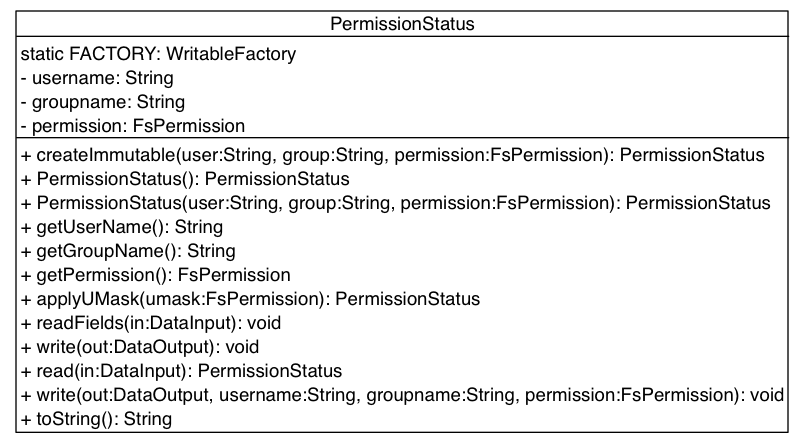
\includegraphics[width=10cm]{cdig/PermissionStatus.png}
     
 存储与权限有关的状态信息.
 提供了与FsPermission对应的权限状态信息

    \begin{XeMethod}{\XePublic}{PermissionStatus}{createImmutable}
         
 创建不可变的PermissionStatus实例 

    \end{XeMethod}

    \begin{XeMethod}{\XePublic}{String}{getUserName}
         
 Return user name
 获取文件所属者名字

    \end{XeMethod}

    \begin{XeMethod}{\XePublic}{String}{getGroupName}
         
 Return group name
 获取文件所属组的名字

    \end{XeMethod}

    \begin{XeMethod}{\XePublic}{FsPermission}{getPermission}
         
 Return permission
 获取用户对文件的操作权限

    \end{XeMethod}

    \begin{XeMethod}{\XePublic}{PermissionStatus}{applyUMask}
         
 Apply umask.
 应用umask设置权限

    \end{XeMethod}

    \begin{XeMethod}{\XePublic}{void}{readFields}
         
 {@inheritDoc}读取各权限信息

    \end{XeMethod}

    \begin{XeMethod}{\XePublic}{void}{write}
         
 {@inheritDoc}输出各权限信息

    \end{XeMethod}

\end{XeClass}
